\documentclass[fontsize=12pt]{article}
\usepackage[utf8]{inputenc}
\usepackage[T1]{fontenc}
\usepackage[german]{babel}
\usepackage{amsmath}
\usepackage{amsthm}
\usepackage{amsfonts}
\usepackage{amssymb}
\usepackage{minted}
\usepackage{tikz}
\usepackage{pgfplots}
\usepackage[top=2cm, bottom=2cm, left=2cm, right=2cm, headheight=1.5cm]{geometry}
\usepackage{fancyhdr}
\usepackage{mdframed}
\usemintedstyle{emacs}

\definecolor{purp}{HTML}{9A72AC}
\definecolor{re}{HTML}{FC6255}
\definecolor{gre}{HTML}{83C167}
\definecolor{blu}{HTML}{58C4DD}
\definecolor{shadecolor}{rgb}{0.85,0.85,0.85}
\definecolor{bg}{rgb}{0.95,0.95,0.95}
\setlength{\parindent}{0em} 

\BeforeBeginEnvironment{minted}{\begin{mdframed}[linewidth =2 ,backgroundcolor=bg , linecolor=black, linewidth=0.5]}
\AfterEndEnvironment{minted}{\end{mdframed}}

\newenvironment{defi}[1]{
    \begin{shaded*}
    \textbf{Definition #1} \\
}{
    \end{shaded*}
}

\newcommand{\bsp}{\textbf{Beispiel}:}
%\newcommand{\task}{\textbf{Aufgabe}:}

\newcommand{\bol}[1]{\textbf{#1}}
\newcommand{\q}[1]{\glqq #1\grqq}
\newcommand{\DODO}[1]{\textbf{\textcolor{red}{DODO:}} #1 \\ \begin{center}\includegraphics[scale=0.2]{../../media/dodo.jpg} \end{center}}

\newenvironment{task}[1]{
    \begin{shaded*}
    \textbf{Aufgabe #1}:
}{
    \end{shaded*}
}



\fancypagestyle{firstpage}{
    \setlength{\headheight}{2.5cm}
    \setlength{\footskip}{0.25cm}
    \pagestyle{fancy}
    \renewcommand{\headrulewidth}{0.4pt}
    \fancyhf{}
    \fancyhead[L]{\LARGE\textbf{Aggregation und Referenzen}}
    \fancyhead[R]{\Large \textbf{Datum:} \hspace{2cm}}
    \fancyfoot[C]{\thepage}
}
\begin{document}
\thispagestyle{firstpage}
\setlength{\headsep}{12pt}
Neben Arrays ist es ein Wesentliches Ziel dieser Jahrgangsstufe, dass in Projekten mehrere Klassen verwendet werden (in kleinerer Form kam dies bereits in der neunten Klasse bei Klassendiagrammen vor!). \\
Damit Objekte verschiedener Klassen einfacher verknüpft werden können, werden sie häufig als Attribute angelegt - bisher waren Attribute hauptsächliche primitive Datentypen wie boolean, int oder double (String war schon die ganze Zeit eine Ausnahme!). \\
Zunächst ein anschaulicheres Beispiel: häufig \q{bestehen} Objekte hauptsächlich aus anderen Objekten (zumindest in der verwendeten Modellierung). Wollen wir beispielsweise ein Stickeralbum modellieren, benötigen wir zwei Klassen, eine für das Album und eine für einen einzelnen Sticker, man kann sagen: das Stickeralbum \textbf{enthält} die Sticker (das entspricht auch der Realität relativ gut!). \\
Im Fachbegriff heißt so eine \q{enthält}-Beziehung \textbf{Aggregation}. Im Objektdiagramm sähe das z.B. so aus: 
\begin{center}
    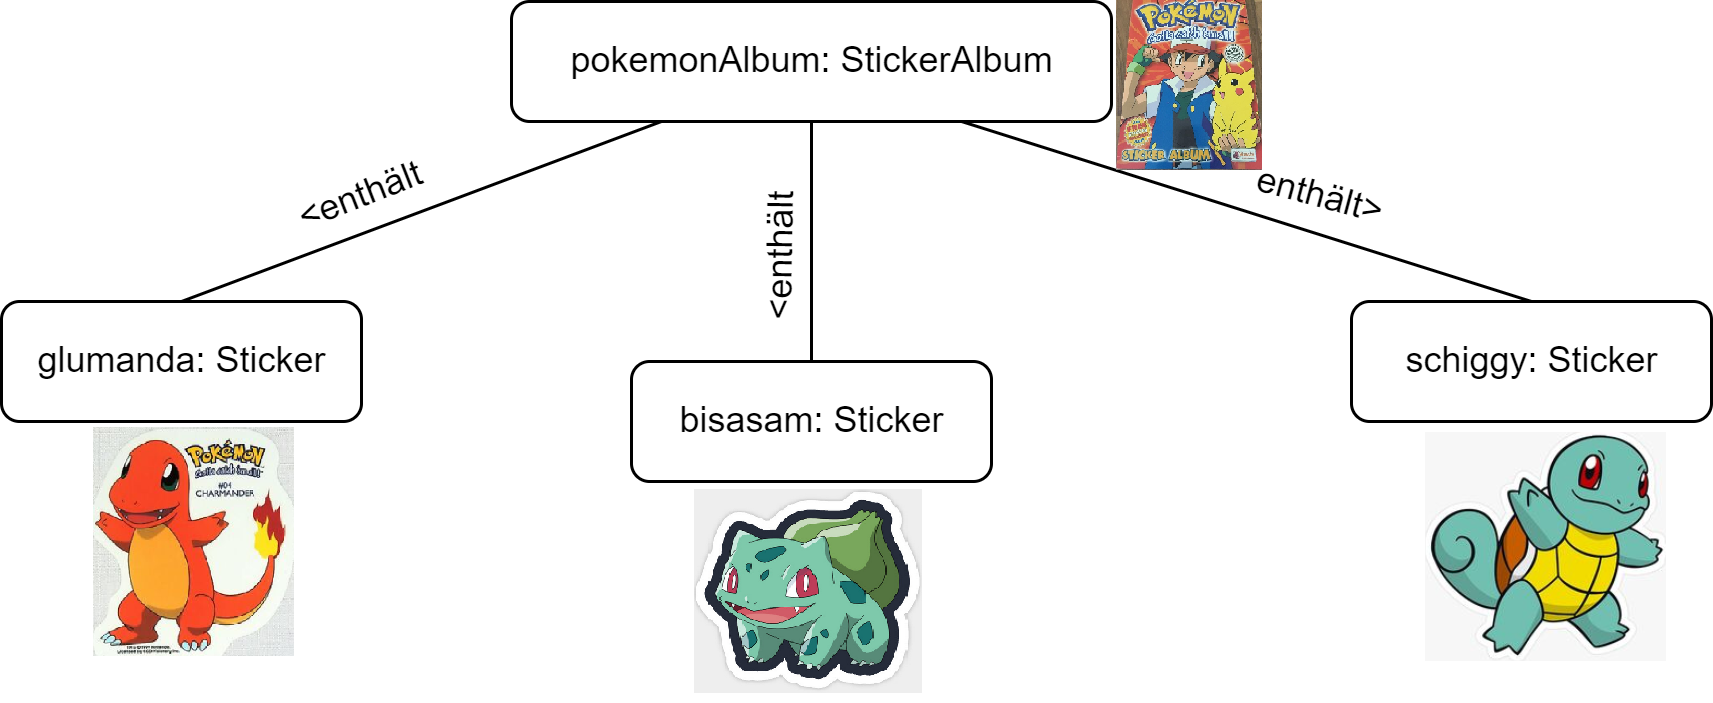
\includegraphics[scale=0.35]{media/obj_diagramm_album.png}
\end{center}
Im Klassendiagramm würde dies mit einem anderen Pfeil markiert werden:
\begin{center}
    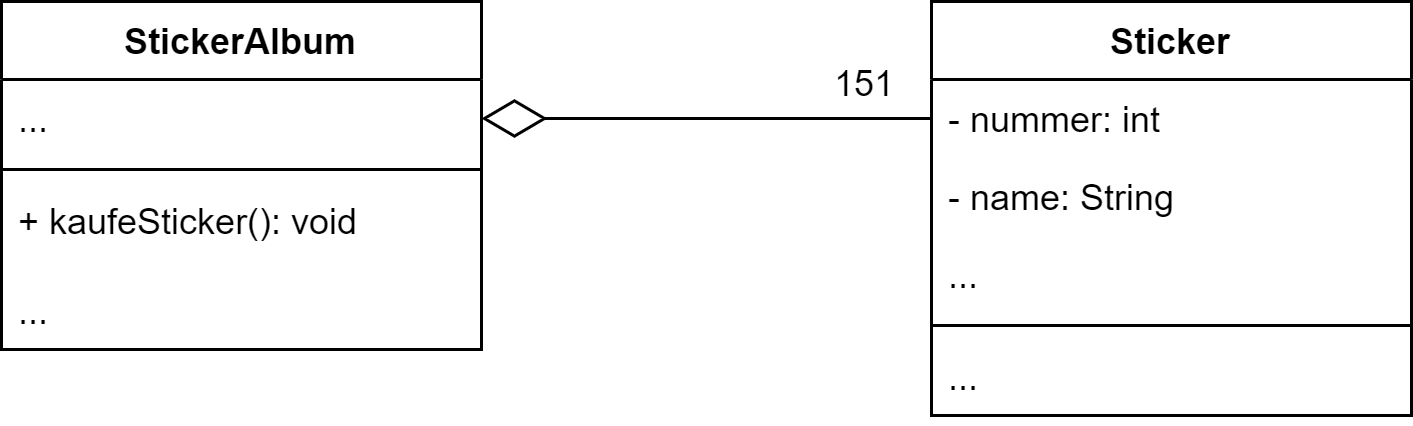
\includegraphics[scale=0.20]{media/class_diagram_album.png}
\end{center}
Ein StickerAlbum besteht also aus 151 Objekten vom Typ Sticker. Die \textbf{Multiplizität} $1$ beim StickerAlbum wird in der Regel weggelassen. Aggregationen werden - wie viele \q{Verbindungen} zwischen Klassen - mit Attributen realisiert. Vereinfachen wir unser Beispiel weiter und nehmen an, dass es nur drei Sticker gibt, dann könnte eine grundlegendeImplementierung des Stickeralbums so aussehen: 
\begin{minted}{java}
public class StickerAlbum {
    private Sticker glumanda;
    private Sticker bisasam;
    private Sticker schiggy;

    public StickerAlbum() {
        bisasam = new Sticker(1, "Bisasam");
        glumanda = new Sticker(4, "Glumanda");
        schiggy = new Sticker(7, "Schiggy");
    }
}
\end{minted}
Dabei wird - wie schon beim Array - mit dem Schlüsselwort \textbf{new} neue Objekte der Klasse Sticker erzeugt. (Man spricht auch von \textbf{Instanziierung)}. \\
\begin{minted}{java}
public class Sticker() {
    int nummer;
    String name;
    public Sticker(int nummer, int name) {
        this.nummer = nummer;
        this.name = name;
    }
}
\end{minted}
\vspace{2mm}
\textbf{Wichtig:} Die Sticker-Objekte sind nicht wirklich im StickerAlbum-Objekt \q{enthalten} im Sinne von: im Speicher stehen sie \q{ineinander}. Vielmehr ist die deklarierte Variable ein Zeiger (Fachbegriff: \textbf{Referenz}), die auf den Ort im Speicher verweist, an dem die eigentlichen Daten abgelegt sind - noch genauer gesagt: auf die Adresse der ersten Speicherzelle, die für das erzeugte Objekt verwendet wird. (im Folgenden noch mit Objektkarten veranschaulicht): \\
\begin{center}
    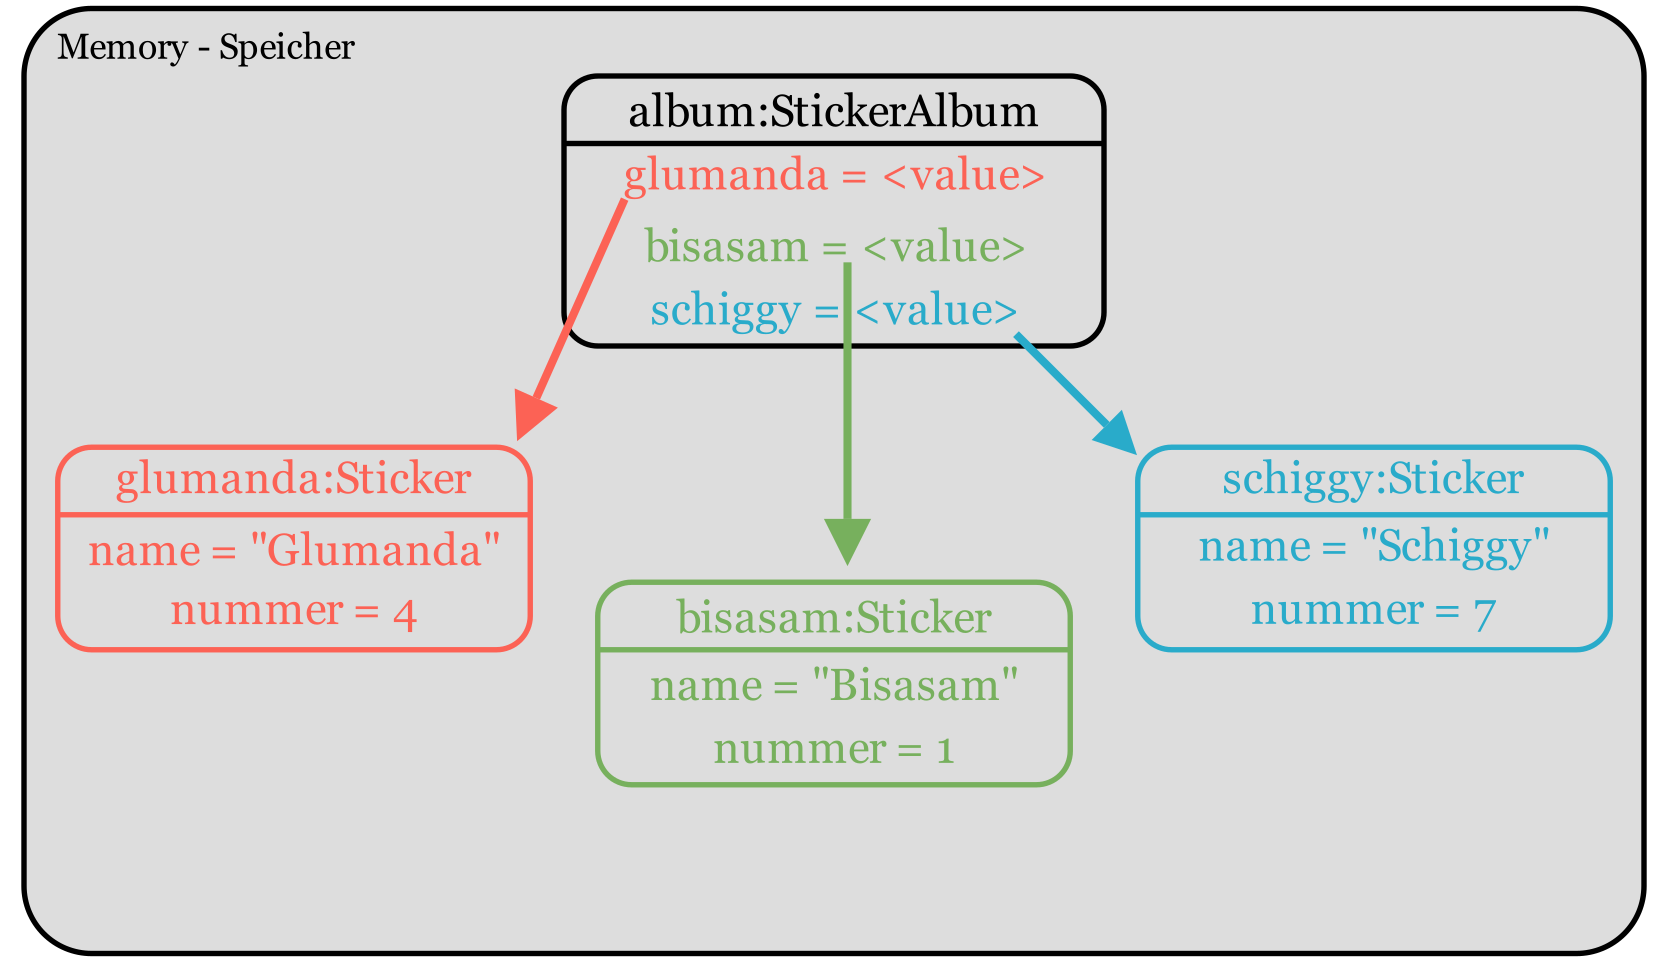
\includegraphics[scale=0.15]{media/speicher_sticker.png}
\end{center}
Ähnliches gilt auch für Arrays. Speichert man primitive Datentypen (also z.B. int, boolean, etc.) in einem Array, so ist die Variable eine Referenz in den Speicher, die an die erste Stelle mit Metadaten zeigt (z.B. liegt dort der Wert des length-Attributs, das wir schon verwendet haben). Anschließend liegen in den folgenden Speicherzellen die Werte explizit abgespeichert. Handelt es sich jedoch um ein Array von Objekten, so ist in jeder der folgenden Speicherzellen nur eine Referenz auf den Speicherort der jeweiligen Objekte vermerkt.
Wären in unserem StickerAlbum von oben die Sticker in einem Array gespeichert, dann sähe Implementierung und Speicherveranschaulichung so aus: 
\begin{minted}{java}
public class StickerAlbum {
    Sticker[] sticker;
    public StickerAlbum() {
        sticker = new Sticker[3];
        sticker[0] = new Sticker(1, "Bisasam");
        sticker[1] = new Sticker(4, "Glumanda");
        sticker[2] = new Sticker(7, "Schiggy");
    }
}
\end{minted}
\begin{center}
    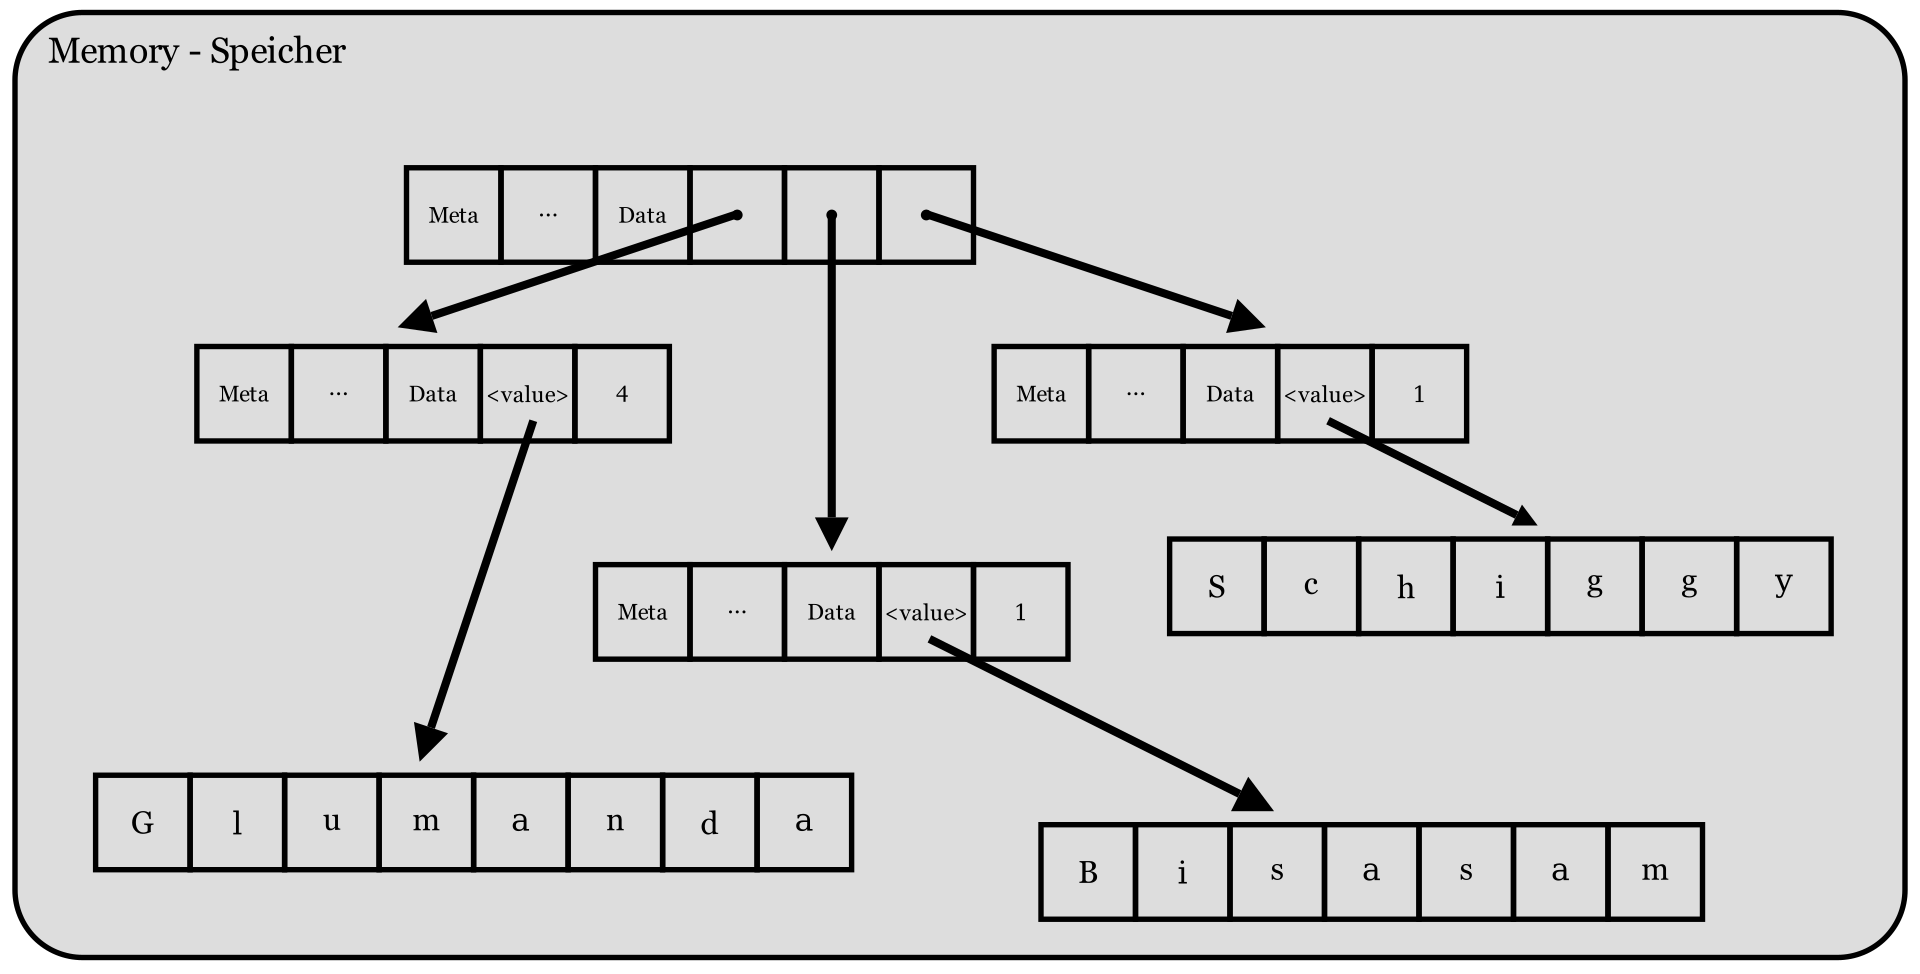
\includegraphics[scale=0.15]{media/speicher.png}
\end{center}
\newpage

Noch einmal zurück zu \textbf{Referenzen}: immer wenn ein Objekt auf ein anderes Objekt \q{verweist} (also nicht nur im Kontext von Arrays) spricht man von einer Referenz. Erst durch diese Referenzen können die Objekte überhaupt miteinander interagieren, da sie ansonsten nichts von der Existenz des jeweils anderen wissen würden. Dabei ergeben sich gewisse Fallstricke. Wir betrachten eine anschauliche Situation, hier als Klassendiagramm:
\begin{center}
    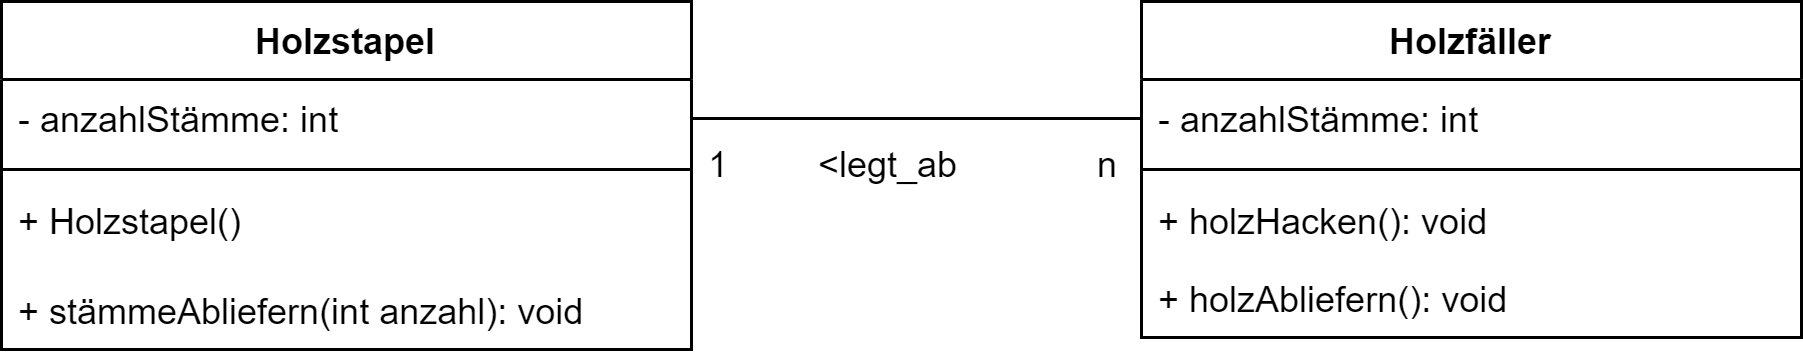
\includegraphics[scale=0.2]{media/class_diagram_holz.png}
\end{center} 
Wir modellieren Holzstapel und Holfzäller. Der Einfachheit halber liefern Holzfäller nur an einem einzigen Stapel ab (deswegen die $1$), allerdings können beliebig viele ($n$) Holzfäller an diesem Stapel ablegen. Eine mögliche Implementierung der beiden Klassen sieht so aus: 
\begin{minted}{java}
public class Holzstapel {
    private int anzahlStämme;
    
    public Holzstapel() {
        anzahlStämme = 0;
    }
    
    public void stämmeAbliefern(int anzahl) {
        if(anzahl <= 0) {
            System.out.println("Das geht so nicht!");
            return;
        }
        anzahlStämme += anzahl;
    }
}
\end{minted}
Im Holzstapel verwalten wir die Anzahl der bereits gefällten Stämme, es können dort nur Stämme abgeliefert werden. 
\begin{minted}{java}
public class Holzfäller {
    private Holzstapel stapel;
    private int anzahlStämme;
    
    public Holzfäller(Holzstapel stapel) {
        anzahlStämme = 0;
        this.stapel = stapel;
    }
    
    public void holzHacken() {
        anzahlStämme++;
    }
    
    public void holzAbliefern() {
        stapel.stämmeAbliefern(anzahlStämme);
        anzahlStämme = 0;
    }
}
\end{minted}
In der Holzfällerklasse können wir entweder Holz hacken (das erhöht die Anzahl der Stämme) oder diese abgeben. Zwei entscheidende Stellen:
\begin{enumerate}
    \item Im Konstruktor wird dieses Mal eine \textbf{Referenz} übergeben, wie oben schon erwähnt wird nicht das komplette Stapel Objekt innerhalb des Holzfällers gespeichert, der Holzfäller \q{kennt} nur seinen Stapel, auf dem er etwas abliefert, d.h. insbesondere, dass \textbf{mehrere} Holzfäller eine Referenz zu \textbf{demselben} Stapel bekommen!
    \item in holzAbliefern() nutzen wir die Punktnotation, um auf dem Holzstapel-Objekt die stämmeAbliefern()-Methode auszuführen. 
\end{enumerate}
Im Fall eines Referenzattributes ist es also nicht unbedingt sinnvoll zu sagen: es handelt sich um eine Eigenschaft der Klasse, so wie wir das bei der Anzahl der Stämme sagen würden. Vielmehr handelt es sich um eine Kommunikationsmöglichkeit. \\
\textbf{Hinweis:} Streng genommen gilt das wie oben erwähnt auch für Strings, da diese selbst auch Objekte sind, hier ist die Bedeutung aber noch näher an der \q{Eigenschaft} als im Fall unseres Holzstapels. \\
Als Veranschaulichung betrachten wir noch das Objektdiagramm, das den Zustand nach folgenden Methodenaufrufen beschreibt:
\begin{minted}{java}
Holzstapel stapel = new Holzstapel();
Holzfäller peter = new Holzfäller();
Holzfäller sandra = new Holzfäller();
peter.holzHacken();
peter.holzHacken();
sandra.holzHacken();
sandra.holzHacken();
sandra.holzAbliefern();
\end{minted}
\begin{center}
    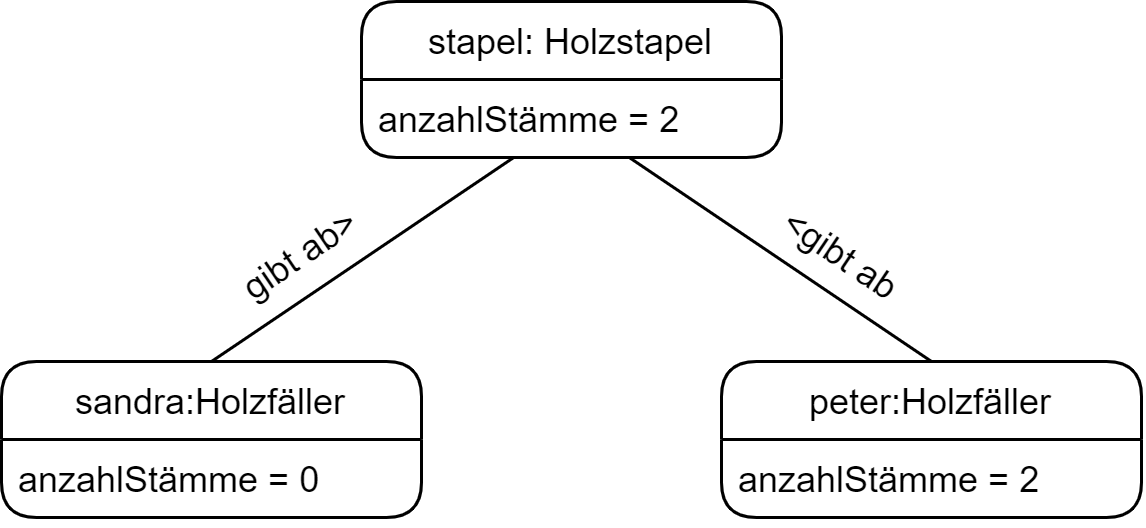
\includegraphics[scale=0.2]{media/obj_diagram_holz.png}
\end{center}
\textbf{Achtung:} Auch Peter hält eine Referenz auf dasselbe Stapel-Objekt wie Sandra, d.h. auch wenn nur Sandra ihre Stämme abgeliefert hat, könnte Peter abrufen, ob bereits Stämme vorhanden sind (wenn es z.B. eine gibAnzahl()-Methode gäbe). \vspace{2mm}\\
\textbf{Gleichartig vs. Identisch}: \\
In unserer Modellierung gibt es direkt nach der Erzeugung zwischen Peter und Sandra eigentlich keinen Unterschied, die Referenzen heißen zwar unterschiedlich, aber beide sind Objekte der Klasse Holzfäller mit einem Attribut \q{anzahlStämme}, das den Wert $0$ hat. D.h. beide sind gleichartig (alle Attributwerte stimmen überein), sie sind aber nicht identisch, da dennoch auf zwei \textbf{verschiedene} Objekte verwiesen wird, deswegen würde der Code
\begin{minted}{java}
    System.out.println(peter == sandra);
\end{minted}
auch den Wert \q{false} auf die Konsole geben, obwohl beide die gleichen Attributwerte haben (die anzahlStämme mit 0 und die Referenz auf denselben Stapel!). Das \textbf{==} vergleicht in Java bei Objekten also nur Referenzen und prüft nicht auf Gleichheit von Attributwerten! Das ist besonders gemein bei Strings:
\begin{minted}{java}
    String a = "abc";
    String b = a;
    String c = "abc";
    String d = new String("abc");
    System.out.println(a == b);
    System.out.println(a == c);
    System.out.println(a == d);
\end{minted}
Dieser Code liefert zweimal \q{true} und einmal \q{false}. Bei $b$ setzen wir einfach eine zweite Referenz, die auf \textbf{dasselbe} String-Objekt zeigt. Bei $c$ dagegen \q{versteht} Java von selbst, dass es sich um denselben String handeln soll und legt gar kein neues Objekt an! Wenn wir Java aber \q{zwingen} (wie bei $d$), dass ein neues String-Objekt angelegt wird, dann ist der entsprechende Vergleich auch \q{falsch}, da die beiden Referenzen an unterschiedliche Stellen im Speicher zeigen. 

\newpage 

\huge\textbf{Assoziationen und Klassendiagramme}\normalsize \\

Bisher haben wir hauptsächlich \textbf{Aggregationen} zur Beschreibung verwendet, nicht immer ganz zutreffend. Zur Erinnerung: eine Aggregation entspricht einer \q{enthält} - Beziehung zwischen zwei Objekten. Bei den Holfzfällern und den Holzstapeln ist das eigentlich nicht ganz zutreffend. Die Objekte kommunizieren zwar miteinander, aber ein Holzfäller \q{besteht} nicht aus einem Holzstapel oder umgekehrt. Die bessere Variante eine solche Beziehung zu beschreiben ist eine einfache \textbf{Assoziation}, repräsentiert durch eine einfache Linie zwischen den beiden Klassen. Man kann auch hier durch \textbf{Multiplizitäten} angeben, auf wie viele Objekte der jeweiligen Klasse zugegriffen wird. \\
\textbf{Beispiel}: 
\begin{center}
    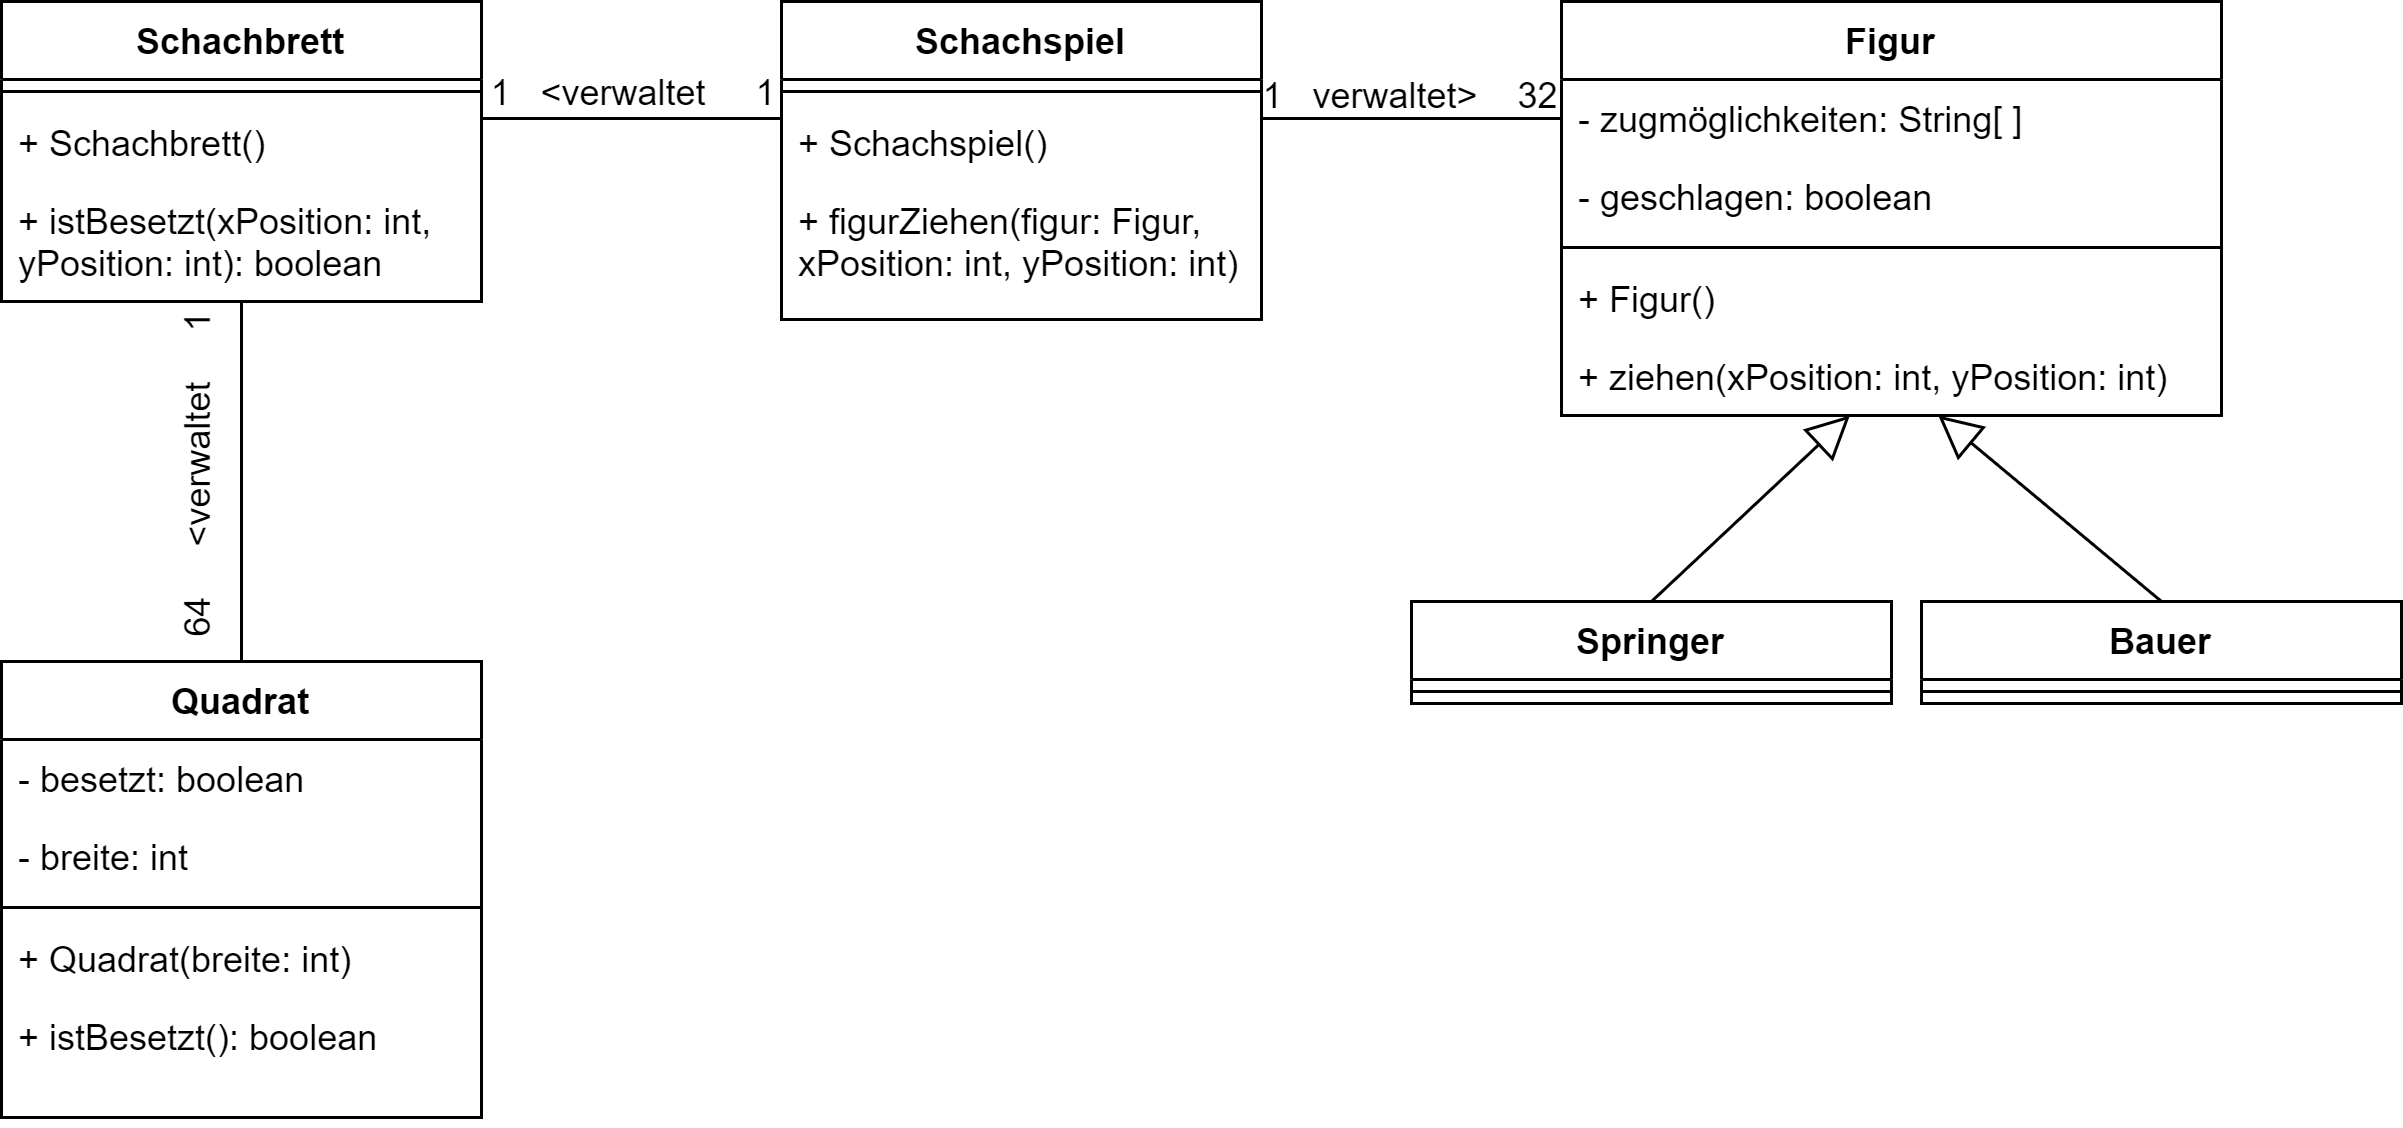
\includegraphics[scale=0.18]{media/class_diagram_associations.png}
\end{center}
Wir betrachten eine - sehr einfache - Variante eines Schachspiels (das Spiel wäre so natürlich noch nicht vollständig funktional, aber für uns ist es ausreichend, für die Profi-Programmierer: das Design ist so auch nicht wirklich geschickt, aber anschaulich :)). \vspace{2mm}\\
Die zentrale Klasse ist das \textbf{Schachspiel}, ein Nutzer soll in dieser Implementierung nur mit dem Schachspiel interagieren (hier kann der Nutzer nur Figuren ziehen und schlagen).\vspace{2mm} \\
Gehen wir davon aus, dass wir unser Schachbrett wieder grafisch mit einem Canvas ausgeben wollen (hier weggelassen), dann muss ein Objekt der Klasse Schachspiel natürlich ein Schachbrett \q{kennen}, hier repräsentiert durch eine \textbf{1:1-Assoziation}. \vspace{2mm} \\
Für die Implementierung ist auch die Bezeichnung und besonders die Pfeilspitze mit der Leserichtung auf der Assoziationslinie wichtig. Hier soll dargestellt werden, dass das Schachspiel das Schachbrett verwaltet, d.h. es gibt nur eine Referenz im Objekt der Klasse Schachspiel auf ein Objekt der Klasse Schachbrett und nicht umgekehrt!\vspace{2mm} \\
Genauso muss das Schachspiel aber z.B. auch die Figuren kennen (hier als Oberklasse Figuren implementiert, neben dem Springer und dem Bauer muss es natürlich noch weitere Unterklassen geben). Da es mehrere Figuren gibt und nicht nur eine, handelt es sich hier um eine \textbf{1:n - Assoziation} (analog zu Datenbanken!), die man in unserem Fall noch präziser angeben kann, da klar ist, dass es nur 32 Figuren im Standard-Schach gibt. Auch hier gilt wieder: das Schachspiel muss auf die Figuren zeigen, um sie \q{ziehen} oder \q{schlagen} zu können. Umgekehrt ist dies aber nicht der Fall! Eine mögliche Implementierung wäre also, ein Feld der Länge 32 im Schachspiel anzulegen. \vspace{2mm} \\
Theoretisch sind auch \textbf{n:m-Assoziationen} möglich, diese sind (gerade bei unseren \q{einfachen} Programmen) aber deutlich seltener  und sollen deswegen nicht vertieft werden. \\
\textbf{Hinweise:}
\begin{itemize}
    \item Auch wenn es im tatsächlichen Code ein Referenzattribut gibt, z.B. vom Schachspiel zum Schachbrett (also \textit{Schachbrett brett;}), so wird dies nicht extra im Diagramm als Attribut angegeben, da die Kante diese Information schon trägt.
    \item Im Wesentlichen sagen die Kanten (und die Pfeilspitzen) aus, welches Objekt auf anderen Objekten der entsprechenden Klassen Methoden aufrufen oder Attribute verändern kann. 
\end{itemize}
\newpage

\textbf{Aufgabe: (Erstellung von Klassendiagrammen und Implementierung)} \\
\textbf{a)} Erstelle ein Klassendiagramm, das folgende Vorgaben beachtet: 
\begin{itemize}
    \item Es soll vier Klassen geben: Bibliothek, Besucher, Buch, Regal.
    \item Die Bibliothek besteht aus 64 Regalen mit Büchern und hat einen Namen. 
    \item Ein Buch wird eindeutig durch seine ISBN-Nummer bestimmt (vereinfacht hier als int dargestellt) und ein Attribut, in dem die Mitgliedsnummer des Besuchers gespeichert wird, der es gerade ausgeliehen hat. Von einem Buch gibt es immer nur ein Exemplar. (Der Inhalt des Buches wird der Einfachheit halber nicht dargestellt!)
    \item Ein Regal enthält 32 Bücher und eine eindeutige Regalnummer. 
    \item Ein Besucher hat einen Namen und eine Mitgliedsnummer in der Bibliothek. Außerdem kann er bis zu sechs Bücher gleichzeitig ausleihen. Er \q{weiß} natürlich welche!
    \item Ein Besucher kann über die Bibliothek ein Buch ausleihen, dazu muss die Bibliothek in den verschiedenen Regalen nach dem Buch \q{suchen}. Dann wird das Buch \q{ausgeliehen} - durch Setzen der entsprechenden Werte im Buch und beim Besucher!
\end{itemize} 
\textbf{b)} Implementiere dein Klassendiagramm!
\end{document}